\documentclass[a4paper,oneside,leqno,12pt]{book}
\usepackage[a4paper,left=4cm,right=3cm,top=3cm,bottom=3cm,head=0cm,headsep=0cm]{geometry}
\usepackage[utf8]{inputenc}
\usepackage{amsmath}
\usepackage{amssymb}
\usepackage{amsthm}
\usepackage{graphicx}
\usepackage{epstopdf}
\usepackage{inputenc}
\usepackage{mathtools}
\usepackage{geometry}
\usepackage{polski}
\usepackage{float}
\usepackage{graphicx}
\usepackage{epstopdf}
\usepackage{subcaption}
\usepackage{color}
\usepackage{url}
\usepackage{clrscode3e}
\usepackage{algorithmicx}
\usepackage[]{algorithm2e}
\usepackage{enumitem}
\usepackage{multicol}
\usepackage{pdfpages}

%\setlist[enumerate]{itemsep=-1mm}
%\DeclareGraphicsExtensions{.eps}

\linespread{1.25}
\pagestyle{plain}

\theoremstyle{definition} 
\newtheorem{przyklad}{Przykład}[chapter]
\newtheorem{definicja}{Definicja}[chapter]
\theoremstyle{plain}
\newtheorem{twierdzenie}{Twierdzenie}[chapter]
\newtheorem{lemat}{Lemat}[chapter]
\theoremstyle{remark}
\newtheorem{uwaga}{Uwaga}[chapter]
\newtheorem{wniosek}{Wniosek}[chapter]

\SetKwProg{ParFor}{parfor}{}{}

\newcommand\BlockIf[1]{\KwSty{Start If} \\ #1 \\ \KwSty{End If}}
\newcommand\BlockElseIf[1]{\KwSty{Start Else If} \\ #1 \\ \KwSty{End Else If}}
\newcommand\BlockElse[1]{\KwSty{Start Else} \\ #1 \\ \KwSty{End Else}}




\begin{document}
\thispagestyle{empty}
\begin{tabular}{c@{\hspace{15mm}}|@{\hspace{3mm}}l}
\vspace{-31mm}  & \\
\multicolumn{2}{l}{\hspace{-35.5mm}
\includegraphics[scale=0.25]{./images/logoumcs}} \\
\multicolumn{2}{@{\hspace{20mm}}l}{\vspace{-4mm}} \\
\multicolumn{2}{@{\hspace{20mm}}l}{\Large UNIWERSYTET MARII CURIE-SKŁODOWSKIEJ} \\
\multicolumn{2}{@{\hspace{20mm}}l}{\vspace{-4mm}} \\
\multicolumn{2}{@{\hspace{20mm}}l}{\Large W LUBLINIE} \\
\multicolumn{2}{@{\hspace{20mm}}l}{\vspace{-4mm}} \\
\multicolumn{2}{@{\hspace{20mm}}l}{\Large Wydział Matematyki, Fizyki i Informatyki} \\
\multicolumn{2}{@{\hspace{20mm}}l}{\vspace{21mm}} \\
& Kierunek: Matematyka \\
& Specjalność: Informatyczna \\
& \\
& Rafał Szczerski  \\
& nr albumu: 2524659 \\
& \\
& \\
& {\Large\textbf{Równoległe algorytmy mnożenia macierzy}} \\
& Parallel matrix multiplication algorithms \\
& \\
& \\
& \\
& \\
& \\
& \\
& Praca licencjacka \\
& \vspace{-7mm} \\
& napisana w Zakładzie Informatyki \\
& \vspace{-7mm} \\
& pod kierunkiem dr Beaty Byliny \\
\multicolumn{2}{@{\hspace{20mm}}l}{\vspace{8mm}} \\
\multicolumn{2}{@{\hspace{20mm}}l}{\textbf{Lublin rok \the\year}}
\end{tabular}
\newpage
\tableofcontents

\chapter{Wstęp}
%\section{Motywacja}
%Można wyróżnić trzy zasadnicze powody obecnego zainteresowania obliczeniami równoległymi.
%\begin{enumerate}
%\item{Stały spadek kosztów sprzętu komputerowego,}
%\item{Rozwój VLSI (\emph{Very-large-scale integration}) do poziomu umożliwiającego projektowanie układów scalonych zawierających miliony tranzystorów na pojedyńczym chipie,}
%\item{Osiągnięcie fizycznych ograniczeń czasu cyklu procesora w architekturze von Neumanna.}
%\end{enumerate}
%
%Obliczenia równoległe, w świetle ograniczeń fizycznych procesorów jednordzeniowych, są odpowiedzią na potrzebę wykonywania szybszych obliczeń. Szybsze obliczenia pozwalają na obliczenia w większej skali i otrzymywanie szybszych rozwiązań.
\chapter{Wiadomości wstępne}
\section{Ustalenia terminologiczne}
\begin{definicja}[Zbiór przechodni]\label{def:transitive_set}
Zbiór \(A\) nazywamy \textbf{przechodnim}, wtedy i tylko wtedy, gdy
\(\forall{x}\left(x\in A \land y\in x\implies y\in A\right)\).  
\end{definicja}

\begin{definicja}[Domknięcie przechodnie zbioru]\label{def:transitive_closure_set}
Domknięciem przechodnim zbioru \(X\) nazywamy najmniejszy w sensie inkluzji zbiór przechodni, który zawiera \(X\).
\end{definicja}

\begin{definicja}[Graf skierowany (DG)]\label{def:DG}
Powiedzmy, że:
\begin{enumerate}
\item \(V\neq\emptyset\) jest zbiorem
\item \( E \subseteq V \times V \)
\end{enumerate}
Grafem skierowanym \(G\) nazwiemy dwójkę \((V, E)\).
\end{definicja}

\begin{definicja}[Acykliczny graf skierowany (DAG)]\label{def:dag}
Acyklicznym grafem skierowanym nazywamy graf skierowany nie zawierający cykli.
\end{definicja}

\begin{definicja}[Domknięcie przechodnie grafu]\label{def:domk_przechodnie_grafu}
Niech \(G=(V,A)\) będzie grafem skierowanym. Graf skierowany \(G^+=(V,A^{+})\) nazywamy \textbf{domknięciem przechodnim} grafu \(G\), gdy \(A^{+}\) jest zbiorem wszystkich takich par \((a,b)\) wierzchołków zbioru \(V\), że w grafie \(G\) istnieje droga z \(a\) do \(b\).
\end{definicja}

\begin{definicja}[Graf zależności]\label{def:depend_graph}
Niech dane będą zbiór \(S\neq\emptyset\), relacja przechodnia \(R\subseteq S\times S\). \textbf{Grafem zależności} nazywamy graf \(G=(S,T)\) i \(T\subseteq R\), gdzie \(R\) jest przechodnim domknięciem \(T\).
\end{definicja}


\begin{definicja}[Ścieżka]\label{def:sciezka}
\textbf{Ścieżką} łączącą \(v_0\) z \(v_n\) o długości \(n\) nazywamy ciąg wierzchołków \((v_0, v_1, \dots, v_n)\) taki, że dla każdego \(k\in \{0, 1, \dots, n-1\}\) istnieje krawędź z \(v_k\) do \(v_{k+1}\).
\end{definicja}

\begin{definicja}[Droga]\label{def:droga}
\textbf{Drogą} w grafie \(G\) nazywamy ścieżkę, której wierzchołki są różne.
\end{definicja}

\begin{definicja}[Długość drogi]\label{def:dlugosc_drogi}
\textbf{Długością} drogi w grafie \(G\) nazywamy liczbę krawędzi, które zawiera droga.
\end{definicja}
\begin{definicja}[Cykl]\label{def:cykl_w_grafie}
Drogę zamkniętą długości co najmniej 1 z ciągiem wierzchołków \(x_1 x_2\dots x_n x_1\) nazywamy \textbf{cyklem}, jeśli wszystkie wierzchołki\\ \(x_1, x_2\dots x_n\) są różne.
\end{definicja}

\begin{definicja}[Stopień wierzchołka]\label{def:stopien_node}
\textbf{Stopień \(d_{G}(v)\) wierzchołka} \(v\) definiujemy jako liczbę incydentnych z \(v\) krawędzi. Każdemu wierzchołkowi \(v\) grafu skierowanego \(G\) możemy przypisać stopień wyjściowy (ang. \emph{indegree}) \(d_{G}^{+}(v)\) i stopień wejściowy (ang. \emph{outdegree}) \(d_{G}^{-}(v)\):
\begin{align*}
 d_{G}^{+}(v) = \#\{w|(v,w)\in E\}\\ 
 d_{G}^{-}(v) = \#\{w|(w,v)\in E\}
\end{align*}
\end{definicja}

\begin{definicja}[Macierz]\label{def:matrix}
Niech \(\mathbb{K}\) będzie ciałem. Macierzą o \(m\) wierszach i \(n\) kolumnach i wartościach w \(\mathbb{K}\) (krótko: macierzą \(m\times n\)) nazwamy każde odwzorowanie \(A:\{1,\dots, m\}\times \{1, \dots, n\}\xrightarrow{} \mathbb{K}, (i,j)\longmapsto A_{ij}\)
\end{definicja}



\newpage

\section{Klasyfikacja algorytmów}

\begin{definicja}[Algorytm]\label{def:algorytm}
Zbiór jednoznacznie określonych reguł lub zadań obliczeniowych prowadzących w skończonej ilości kroków do rozwiązania pewnego problemu \cite{IEEE}.\\
\end{definicja}

Określone w ten sposób zadania obliczeniowe są z reguły względem siebie niezależne. Pewne z nich mogą być wykonywane równolegle, inne -- sekwencyjnie, jedno po drugim. Wobec tego algorytm może być określony częściowo równolegle, częściowo sekwencyjnie.\\

Na podstawie niezależności zadań obliczeniowych algorytmy możemy podzielić na pięć klas \cite{APC2011}:
\begin{enumerate}
\item Algorytmy szeregowe
\item Algorytmy równoległe
\item Algorytmy szeregowo--równoległe (SPA, Serial--Parallel Algorithms)
\item Algorytmy nieszeregowo--równoległe (NSPA, Nonserial--Parallel Algorithms)
\item Algorytmy regularno-iteracyjne (RIA, Regular--Iterative Algorithms)
\end{enumerate}





\begin{definicja}[Algorytm sekwencyjny]\label{def:algorytm_sekwencyjny}
\textbf{Algorytm sekwencyjny} (rys.  \ref{fig:sequential}) jest ciągiem dokładnie sprecyzowanych zadań obliczeniowych \(T_i,\, i\in\mathbb{N}\) rozwiązujących dany problem, tj. wyznaczających dane wyjściowe na podstawie danych wejściowych. Zakłada się, że w algorytmie sekwencyjnym zadania wykonywane są przez jeden procesor.
\end{definicja}

\begin{figure}[h]
\centering
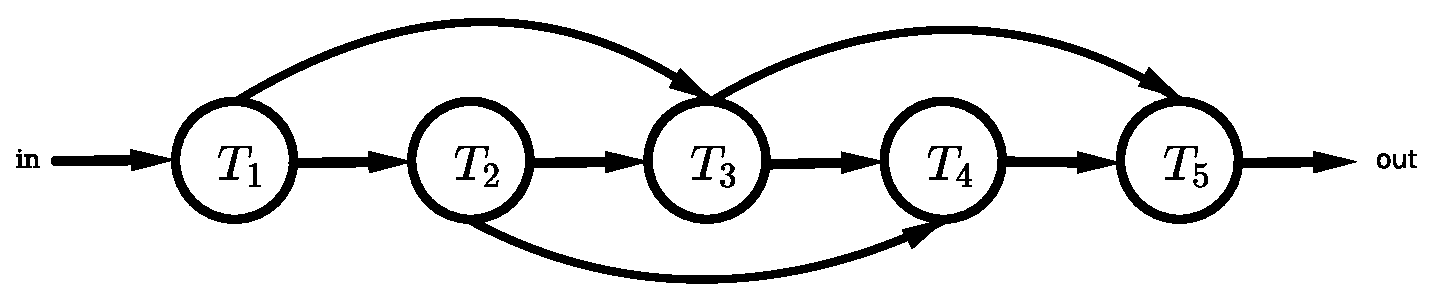
\includegraphics[width=29em]{./images/Rys2.eps}
\caption{Algorytm sekwencyjny}
\label{fig:sequential}
\end{figure}

W celu rozwiązania problemu za pomocą większej liczby procesorów należy go zdekomponować na podproblemy, które mogą być rozwiązane równolegle. Każdy z podproblemów rozwiązywany jest przez odrębny algorytm będący składową algorytmu równoległego.


\begin{definicja}[Równoległość]\label{def:rownoleglosc}
\textbf{Równoległość} w odniesieniu do oprogramowania jest to symultaniczny transfer, występowanie albo przetwarzanie poszczególnych części pewnej całości, takich jak bity składające się na znak albo znaki pewnego słowa, używając osobnych urządzeń dla ich różnych części \cite{IEEE}.
\end{definicja}

\begin{definicja}[Algorytm równoległy]\label{def:algorytm_rownolegly}
\textbf{Algorytmem równoległym} (rys.  \ref{fig:parallel}) nazywamy każdy algorytm w którym spośród określonych w nim zadań \(T_1\), \(T_2\), \(\dots\), \(T_n\) co najmniej dwa zadania \(T_i\), \(T_j\), \(i\neq j\) dzięki ich wzajemnej niezależności, mogą być wykonane równocześnie \cite{APC2011}.\\
\end{definicja}

\begin{figure}[h]
\centering
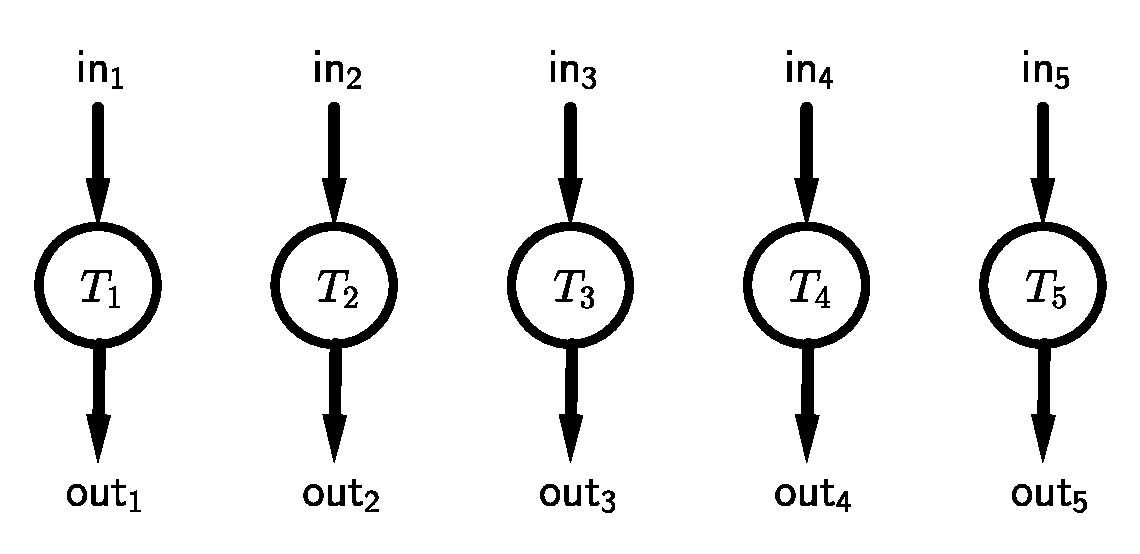
\includegraphics[width=23em]{./images/Rys1.eps}
\caption{Algorytm równoległy}
\label{fig:parallel}
\end{figure}

\begin{definicja}[Architektura równoległa]\label{def:arch_rownolegla}
\textbf{Architektura równoległa} jest to architektura wieloprocesorowa, na której można wykonywać przetwarzanie równoległe \cite{IEEE}.
\end{definicja}

Algorytmy równoległe i architektury równoległe są ze sobą blisko spokrewnione. Równoległość może być zaimplementowana na wielu poziomach używając technik sprzętowych i programowych\cite{APC2011}
\begin{enumerate}
\item{Równoległość na poziomie danych (\emph{Data-level parallelism}), gdzie pracujemy na wielu bitach danych lub na wielu danych jednocześnie.}
\item{Równoległość na poziomie instrukcji (\emph{Instruction-level parallelism}, ILP), gdzie jednocześnie procesor może wykonać więcej niż jedną instrukcję.}
\item{Równoległość na poziomie wątków (\emph{Thread-level parallelism}, TLP). Wątem jest częścią programu, która współdzieli zasoby procesora z innymi wątkami. W TLP wiele programowych wątków jest uruchamianych jednocześnie na jednym bądź wielu procesorach.}
\item{Równoległość na poziomie procesów (\emph{Process-level parallelism}). Proces to program, który jest uruchomiany na komputerze. Rezerwuje on własne zasoby komputera, takie jak przestrzeń pamięciową i rejestry.}
\end{enumerate}

\begin{przyklad}
Prostym przykładem algorytmu równoległego jest serwer siecowy, który każde zapytanie przychodzące przetwarza niezależnie od innych zapytań. Innym przykładem są wielozadaniowe systemy operacyjne, radzące sobie z jednoczesną obsługą kilku uruchomionych programów.
\end{przyklad}
%
%\begin{definicja}[Algorytmy szeregowo--równoległe]
%
%\end{definicja}
%
%\begin{definicja}[Algorytmy nieszeregowo--równoległe]
%\end{definicja}
%
%\begin{definicja}[Algorytmy regularno--iteracyjne]
%Algorytmy tej klasy reprezentowane za pomocą grafów zależności wyrażają pewien pewien ustalny schemat postępowania.
%\end{definicja}

\subsection{Reprezentacja algorytmów}


Wiele obliczeń możemy repezentować za pomocą acyklicznych grafów skierowanych. Każde wejście jest oznaczane przez węzeł bez dochodzących do niego łuków. Operacje oznaczamy przez węzły do których wchodzą łuki z innych węzłów oznaczających argumenty (operandy). Stopień wejściowy dowolnego węzła wynosi co najwyżej 2. Węzeł, którego stopień wyjściowy jest równy 0 oznacza wyjście. Zakładamy, że każdy węzeł przedstawia operację, która wymaga jednej jestostki czasu wykonania.\\



Za pomocą acyklicznych grafów skierowanych możemy analizować zachowanie równoległych algorytmów przy założeniu, że każdy z procesorów ma dostęp do danych obliczonych przez inny procesor bez dodatkoych narzutów. Implementacja algorytmu polega na \emph{planowaniu} wykonania każdego węzła na wybranym procesorze.
%\begin{figure}[h]
%\centering
%\includegraphics[width=34em]{Rys3.eps}
%\caption{Algorytm macierzenia macierzy przedstawiony za pomocą DAG'a}
%\label{fig:example_dag}
%\end{figure}

Powiedzmy, że dla danych \(p\) procesorów, chcemy przyporządkować każdemu węzłowi \(i\) parę \((j_i, t_i)\), gdzie \(j_i \leq p\) oznacza indeks procesora, zaś \(t_i\) jednostkę czasu, taką że zachodzą poniższe warunki:
\begin{enumerate}
\item Jeśli \(t_i=t_k\) dla pewnego \(i\neq k\), to \(j_i\neq j_k\). Oznacza to, że każdy procesor może wykonać pojedyńczą operację podczas każdej jednostki czasu.
\item Jeśli \((i, k)\) jest łukiem grafu, to \(t_k\geq t_i + 1\). Oznacza to, że operacja, którą przedstawia węzeł k powinna być zaplanowania po wykonaniu operacji przedstawionej przez węzeł \(i\).
\end{enumerate}

Przyjmuje się, że czas \(t_i\) węzła wejściowego \(i\) wynosi 0 oraz żaden procesor nie jest przyporządkowany do tego węzła.\\
\begin{definicja}[Plan]\label{def:plan}
Ciąg \(\{(j_i, t_i) | i\in N\}\) nazywamy \textbf{planem} równoległego wykonania DAG przez \(p\) procesorów, gdzie \(N\) oznacza zbiór węzłów DAG.
\end{definicja}
Dla dowolnego planu, odpowiadający mu czas wykonania (złożoność czasowa) algorytmu jest określony przez \(\max_{i\in N}t_i\). Złożonośc równoległa DAG'a jest określona przez \(T_{p}(n) = \min{\{\max_{i\in N}t_i\}}\), gdzie minimum bierzemy po wszystkich planach, które używają \(p\) procesorów.


\begin{przyklad}
Niech \(\mathbf{A}\), \(\mathbf{B}\in\mathbb{R}^{n\times n}\). Rozważmy standardowy algorytm obliczający iloczyn macierzy \(AB = C\). Każdy \(C(i, j)\) obliczamy za pomocą wyrażenia \(C(i, j)=\sum_{l=1}^{n}A(i,l)B(l,j)\). Odpowiadający obliczeniu DAG dla \(n=4\) przedstawia Rys. \ref{fig:standard_parallel}. Mając \(n^3\) procesorów, operacje mogą być zaplanowane poziom po poziomie, używając n procesorów do obliczenia każdego z elementów macierzy wynikowej \(C\). Stąd widać, że możemy zaplanować DAG do obliczenia o złożoności \(O(\log{n})\)
\begin{figure}[H]
\centering
\includegraphics[width=36em]{./images/Rys3.eps}
\caption{Standardowy iloczyn macierzowy}
\label{fig:standard_parallel}
\end{figure}

\end{przyklad}

\section{Ocena algorytmów}
\label{subsec:algorytmy_sekwencyjne}
\subsection{Algorytmy sekwencyjne}

Ograniczenia zasobów (np. czasu i przestrzeni) wymagane przez algorytmy sekwencyjne mierzymy jako funkcję rozmiaru danych wejściowych \(T(n)\), tzw. złożoność czasową. Ograniczenia te wyrażamy asymptotycznie używając notacji:

\begin{enumerate}
\item{\(T(n) = O(f(n))\), jeśli istnieje dodatnie stałe \(c\) i \(n_0\) takie, że \(\forall{n \geq n_0}: (T(n)\leq cf(n)) \)}
\item{\(T(n) = \Omega(f(n))\), jeśli istnieje dodatnie stałe \(c\) i \(n_0\) takie, że \(\forall{n \geq n_0}: (T(n)\geq cf(n)) \)}
\item{\(T(n) = \Theta(f(n))\), jeśli \(T(n)=O(f(n))\) i \(T(n)=\Omega(f(n))\)}
\end{enumerate}
Czas działania algorytmu sekwencyjnego szacuje się przez liczbę operacji podstawowych wymaganych przez algorytm jako funkcję ilości danych wejściowych.
\subsection{Algorytmy równoległe}

Załóżmy że algorytm równoległy \(R\) rozwiązuje problem \(Z\) o rozmiarze \(n\). \textbf{Pesymityczną złożonością czasową algorytmu} \(R\) nazywamy funkcję:\\

\begin{align}
T_{p}(n) = \sup_{d\in{D_n}}{\left\{t(p,d)\right\}},
\end{align}
gdzie \(t(p,d)\) oznacza liczbę kroków obliczeniowych (operacji dominujących) wykonanych dla zestawu danych \(d\) od momentu rozpoczęcia obliczeń algorytmu \(R\) przez pierwszy procesor do chwili zakończenia obliczeń przez wszystkie procesory, \(p\) -- liczbę procesorów, \(D_n\) -- zbiór wszystkich zestawów danych wejściowych \(d\) o rozmiarze \(n\) \cite{Czech}.


\subsection{Przyspieszenie}

Potencjalną korzyść z równoległego wykonania zadania obliczeniowego możemy zmierzyć licząć czas jaki zajmuje wykonanie go na jednym procesorze i porównanie wyniku z wykonaniem tego samego zadania równolegle na \(N\) procesorach. Współczynnik przyspieszenia \(S(p, n)\) możemy zdefiniować jako

\begin{align}\label{def:speedup_abs}
 S(p, n)=\frac{T^{*}_{p}(1)}{T_{p}(N)}
\end{align}

gdzie \(T^{*}_{p}(1)\) jest pesymistyczną złożonością czasową najszybszego znanego algorytmu sekwencyjnego rozwiązującego problem \(Z\) na jednym procesorze, \(T_{p}(N)\) jest pesymistyczną złożonością algorytmu równoległego. Wyrażenie \ref{def:speedup_abs} nazywamy \textbf{przyspieszeniem bezwzględnym}.

Maksymalną wartością przyspieszenia \(S(p,n)\) jest p, ponieważ używając \(p\) procesorów można przyspieszyć obliczenia najlepszego algorytmu sekwencyjnego co najwyżej \(p\) razy. Zwykle uzyskiwane przyspieszenie jest mniejsze niż \(p\). Przyczyną tego może być niewystarczający stopień współbieżności w problemie \(Z\). 



W złożoności \(T^{r}_{1}(n)\) można wyróżnić operacje obliczeniowe, które muszą być wykonane sekwencyjnie, \(T^{s}_{1}(n)\), oraz obliczenia, które mogą być wykonane równolegle, \(T^{r}_{1}(n)\). Wobec tego mamy, że:

\begin{align}
T_{1}(n) = T^{s}_{1}(n) + T^{r}_{1}(n)
\end{align}

Zakładając, że obliczenia \(T^{r}(n)\) da się równomiernie rozdzielić między \(p\) procesorami, przyspieszenie \(S(p, n)\) wyraża się wzorem:

\begin{align}\label{eq:supSpn}
S(p, n) = \frac{T_{1}(n)}{T_{p}(n)}\leq\frac{T^{s}_{1}(n) + T^{r}_{1}(n)}{T^{s}_{1}(n) + T^{r}_{1}(n)/p + T^{o}_{p}(n)}
\end{align}


gdzie \(T^{o}_{p}(n)\) jest złożonością dodatkową wynikającą z organizacji obliczeń równoległych. W jej skład wchodzą m.in. operacje komunikacji między procesorami.




\subsection{Prawo Amdahla}

Rozważmy algorytm sekwencyjny o złożoności \(T_1(n)\) rozwiązujący zadany problem o dowolnym, ustalonym rozmiarze \(n\). Niech \(s\) oznacza część obliczeń algorytmu, która musi być wykonana sekwencyjnie, zaś \(r\) część obliczeń, która może być wykonana równolegle. Mamy wówczas: \(T^{s}(n) = sT_{1}(n), T^{r}(n)=rT_{1}(n)\), gdzie \(s+r=1\). Przyspieszenie algorytmu, jakie można uzyskać po jego zrównolegleniu można wyznaczyć upraszczając wzór \eqref{eq:supSpn} przez pominięcie złożoności \(T^{o}_{p}(n)\).

Mamy wówczas:
\begin{equation}\label{eq:amdahl}
\begin{split}
S(p, n) &= \frac{T_{1}(n)}{T_{p}(n)}\leq\\
&\leq \frac{T^{s}_{1}(n) + T^{r}_{1}(n)}{T^{s}_{1}(n) + T^{r}_{1}(n)/p + T^{o}_{p}(n)}\leq\\
&\leq \frac{sT_{1}(n) + rT_{1}(n)}{sT_{1}(n) + rT_{1}(n)/p} =
= \frac{s+r}{s+r/p} = \frac{1}{s+r/p}= \\
&= \left(s+\frac{1-s}{p}\right)^{-1}
\end{split}
\end{equation}
gdzie \(s\) – część obliczeń w algorytmie które muszą być wykonane sekwencyjnie; \(p\) – liczba procesorów.\\

Wzór \eqref{eq:amdahl} znany jest jako \textbf{prawo Amdahla}. Służy on do wyznaczania górnego ograniczenia przyspieszenia będącego funkcją \(s\) oraz liczby procesorów \(p\) przy ustalonym rozmiarze problemu \(n\).


\subsection{Prawo Gustafsona i Barsisa}

Niech \(p\) oznacza liczbę procesorów, \(\sigma\) -- część czasu obliczeń algorytmu równoległego przypadającą na wykonanie obliczeń w sposób sekwencyjny, a \(\rho\) -- część czasu obliczeń algorytmu równoległego przypadającą na wykonywanie obliczeń w sposób równoległy takie, że \(\sigma+\rho=1\). Czas wykonania tego samego algorytmu w hipotetycznym komputerze sekwencyjnym jest proporcjonalny do sumy \(\sigma + p\rho\), gdzie wyrażenie \(p\rho\) odpowiada czasowi wykonania części równoległej obliczeń przez jeden procesor. Przyspieszenie, które zostałoby uzyskane, gdyby obliczenia równoległe zostały przeprowadzone w komputerze sekwencyjnym wyraża się przez:
\begin{equation}\label{eq:gustafson&barsis}
\Psi(p,n)\leq\frac{\sigma+p\rho}{\sigma+\rho}=\sigma+p\rho=\sigma+p\left(1-\sigma\right)=p+\left(1-p\right)\sigma
\end{equation}

Wzór \eqref{eq:gustafson&barsis} jest znany jako \textbf{prawo Gustafsona i Barsisa}. Definiuje ono tzw. \textbf{skalowane przyspieszenie}, ponieważ wraz ze zmianą liczby procesorów skaluje się odpowiednio rozmiar problemu, tak aby utrzymać stały czas obliczeń równoległych \cite{Czech}.

\newpage


\section{Teoretyczne modele obliczeń }
\subsection{Model RAM}
Nim przejdziemy do omówienia modeli obliczeń równoległych zajmiemy się omówieniem modelu RAM zwanego również architekturą von Neumanna.

Model RAM (\emph{Random Access Machine}) odpowiada rozważaniom zawartym w \ref{subsec:algorytmy_sekwencyjne}. Zakłada on:

\begin{enumerate}
\item{Istnienie pewnego procesora wyposażonego w:
\begin{enumerate}
\item skończoną listę instrukcji, które może on realizować
\item pewną liczbę rejestrów arytmetycznych procesora \(R_1, R_2, \dots, R_n\), \(n>1\) które mogą przechowywać dowolne skończone liczby w zapisie binarnym
\item specjalny rejestr sterujący \(L\) zwany licznikiem programu.
\end{enumerate}}
\item Istnienie pamięci złożonej z potencjalnie nieskończonej liczby komórek \(M_i, \, i=1, 2, 3, \dots\) (Rys. \ref{fig:ram}) w których można przechowywać dowolną skończoną liczbę w zapisie binarnym.
\item Stały czas zapisu i odczytu wartości do/z komórki pamięci (inaczej \emph{dostęp swobodny}).

\end{enumerate}

\begin{figure}[h]
\centering
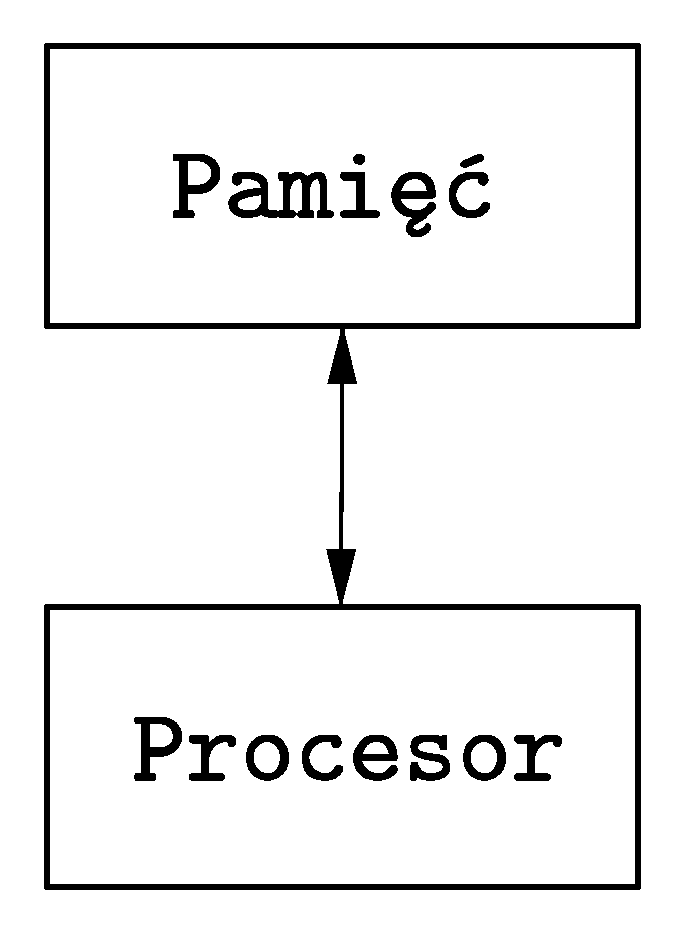
\includegraphics[width=7em]{./images/Rys_RAM.eps}
\caption{Model obliczeń sekwencyjnych RAM}
\label{fig:ram}
\end{figure}

\begin{table}[H]
\begin{center}
\caption{Przykładowa lista instrukcji procesora\cite{Czech}}
\label{tab:ram_instructions}
\begin{tabular}{|l|c|l|}
\hline
Instrukcja & Argument & Znaczenie \\ \hline
\texttt{LOAD} & \(k, a\) & \(R_k:=w(a)\) \\
\texttt{STORE} & \(k, b\) & \(M_{w(b)}:=R_{k}\) \\
\texttt{ADD} & \(k, c\) & \(R_{k}:=R_{k}+w(c)\) \\
\texttt{SUB} & \(k, c\) & \(R_{k}:=R_{k}-w(c)\)\\
\texttt{MULT} & \(k, c\) & \(R_{k}:=R_{k} \times w(c)\)\\
\texttt{DIV} & \(k, c\) & \(R_{k}:=\lfloor R_{k}/w(c)\rfloor\) \\
\texttt{JUMP} &  \(i\) & \(L:=i\) \\
\texttt{JPOS} & \(k,i\) & \texttt{if} \(R_k>0\) \texttt{then} \(L:=i\) \texttt{else} \(L:=L+1\) \\
\texttt{JZERO} & \(k,i\) & \texttt{if} \(R_k==0\) \texttt{then} \(L:=i\) \texttt{else} \(L:=L+1\) \\
\texttt{JNEG} & \(k,i\) & \texttt{if} \(R_k<0\) \texttt{then} \(L:=i\) \texttt{else} \(L:=L+1\) \\
\texttt{READ} & k & Wczytaj daną z urządzenia zewnętrznego do rejestru \(R_k\) \\
\texttt{WRITE} & k & Wydrukuj daną z rejestru \(R_k\) \\
\texttt{HALT} & & Zakończ obliczenie \\ \hline
\end{tabular}
\end{center}
\end{table}


\label{subsec:PRAM}
\subsection{Model PRAM}

Model wspólnej pamięci składa się z pewnej liczby procesorów, z których każdy posiada własną pamięć i może lokalnie wykonywać programy. Wszystkie procesory mogą komunikować się za pomocą wspólnej globalnej pamięci.\\
Każdemu procesorowi przypożądkowany jest niepowtarzająca się liczba naturalna. Jest to lokalnie dostępny indeks, numer procesora lub jego identyfikator.\\

W modelu wspólnej pamięci wyróżniamy dwa podstawowe tryby operacji. W pierwszym trybie, synchronicznym, wszystkie procesory działają synchronicznie według wspólnego zegara. Model ten nazywamy równoległą maszyną o dostepie swobodnym (PRAM, parallel random-access machine).\\
W drugi trybie, asynchronicznym, każdy procesor pracuje według osobnego zegara. W tym trybie programista jest odpowiedzialny za odpowiednią synchronizację procesorów, jeśli zachodzi taka potrzeba. Dokładniej mówiąc, jeśli procesor ma pobrać dane, to odpowiedzialnością programisty jest upewnienie się, że odpowiednie dane są już uzyskane, ponieważ wartości wspólnych zmiennych są określane dynamicznie w trakcie wykonania programu na różnych procesorach.\\

Ponieważ każdy procesor może uruchomić swój program lokalnie, ten model jest typu MIMD w klasyfikacji Flynna. Znaczy to tyle, że każdy procesor może wykonać pewną instrukcję lub operację na danych niezależnie od tych wykonanych na jakimkolwiek innym procesorze w trakcie danej jednostki czasu.\\

Dla danego algorytmu, rozmiar danych wymienionych pomiędzy pamięcią globalną i pamięcią lokalną różnych procesorów wyraża rozmiar \textbf{komunikacji} wymaganej przez algorytm.



Możemy wyróżnić kilka wariantów modelu PRAM w zależności od wymagań jakie postawimy odnośnie jednoczesnego dostępu kilku procesorów do tego samego adresu w pamięci globalnej.\\
\begin{definicja}{Klasyfikacja PRAM ze względu na dostęp do pamięci}
\begin{itemize}
\item\textbf{EREW} -- algorytmy z wyłącznym odczytem i wyłącznym zapisem; nie pozwala na jednoczesny zapis do pamieci\\
\item\textbf{CREW} -- algorytmy z jednoczesnym odczytem i wyłącznym zapisem; pozwala na jednoczesny  dostęp do pamięci dla instrukcji odczytu\\
\item\textbf{CRCW} -- algorytmy z jednoczesnym odczytem i jednoczesnym zapisem;\\
\item\textbf{ERCW} -- algorytmy z wyłącznym odczytem i jednoczesnym zapisem.\\
\end{itemize}
\end{definicja}

Jeśli nie poczyni się żadnych dodatkowych założeń, to nie jest jasno określone, co zostanie zapisane w komórce pamięci w wyniku jednoczesnego zapisywania do niej przez wiele procesorów w algorytmie typu CRCW. W literaturze można spotkać wiele typów maszyny PRAM, które różnią się sposobami rozwiązywania konfliktów zapisu. Można wśród nich wyróżnić\cite{Cormen94}:

\begin{enumerate}
\item jednolity (ang. common) – procesory muszą zapisać do tej samej komórki pamięci jednolitą wartość
\item dowolny (ang. arbitrary) – zapamiętywana jest dowolna wartość z wartości zapisywanych do tej samej komórki pamięci
\item priorytetowy (ang. priority) – zapamiętywana jest wartość zapisywana przez procesor o najmniejszym numerze
\item (ang. combining) – zapamiętywana jest wartość jest pewną, jednak ściśle określoną kombinacją zapisywanych wartości
\end{enumerate}

\begin{figure}[h]
\centering
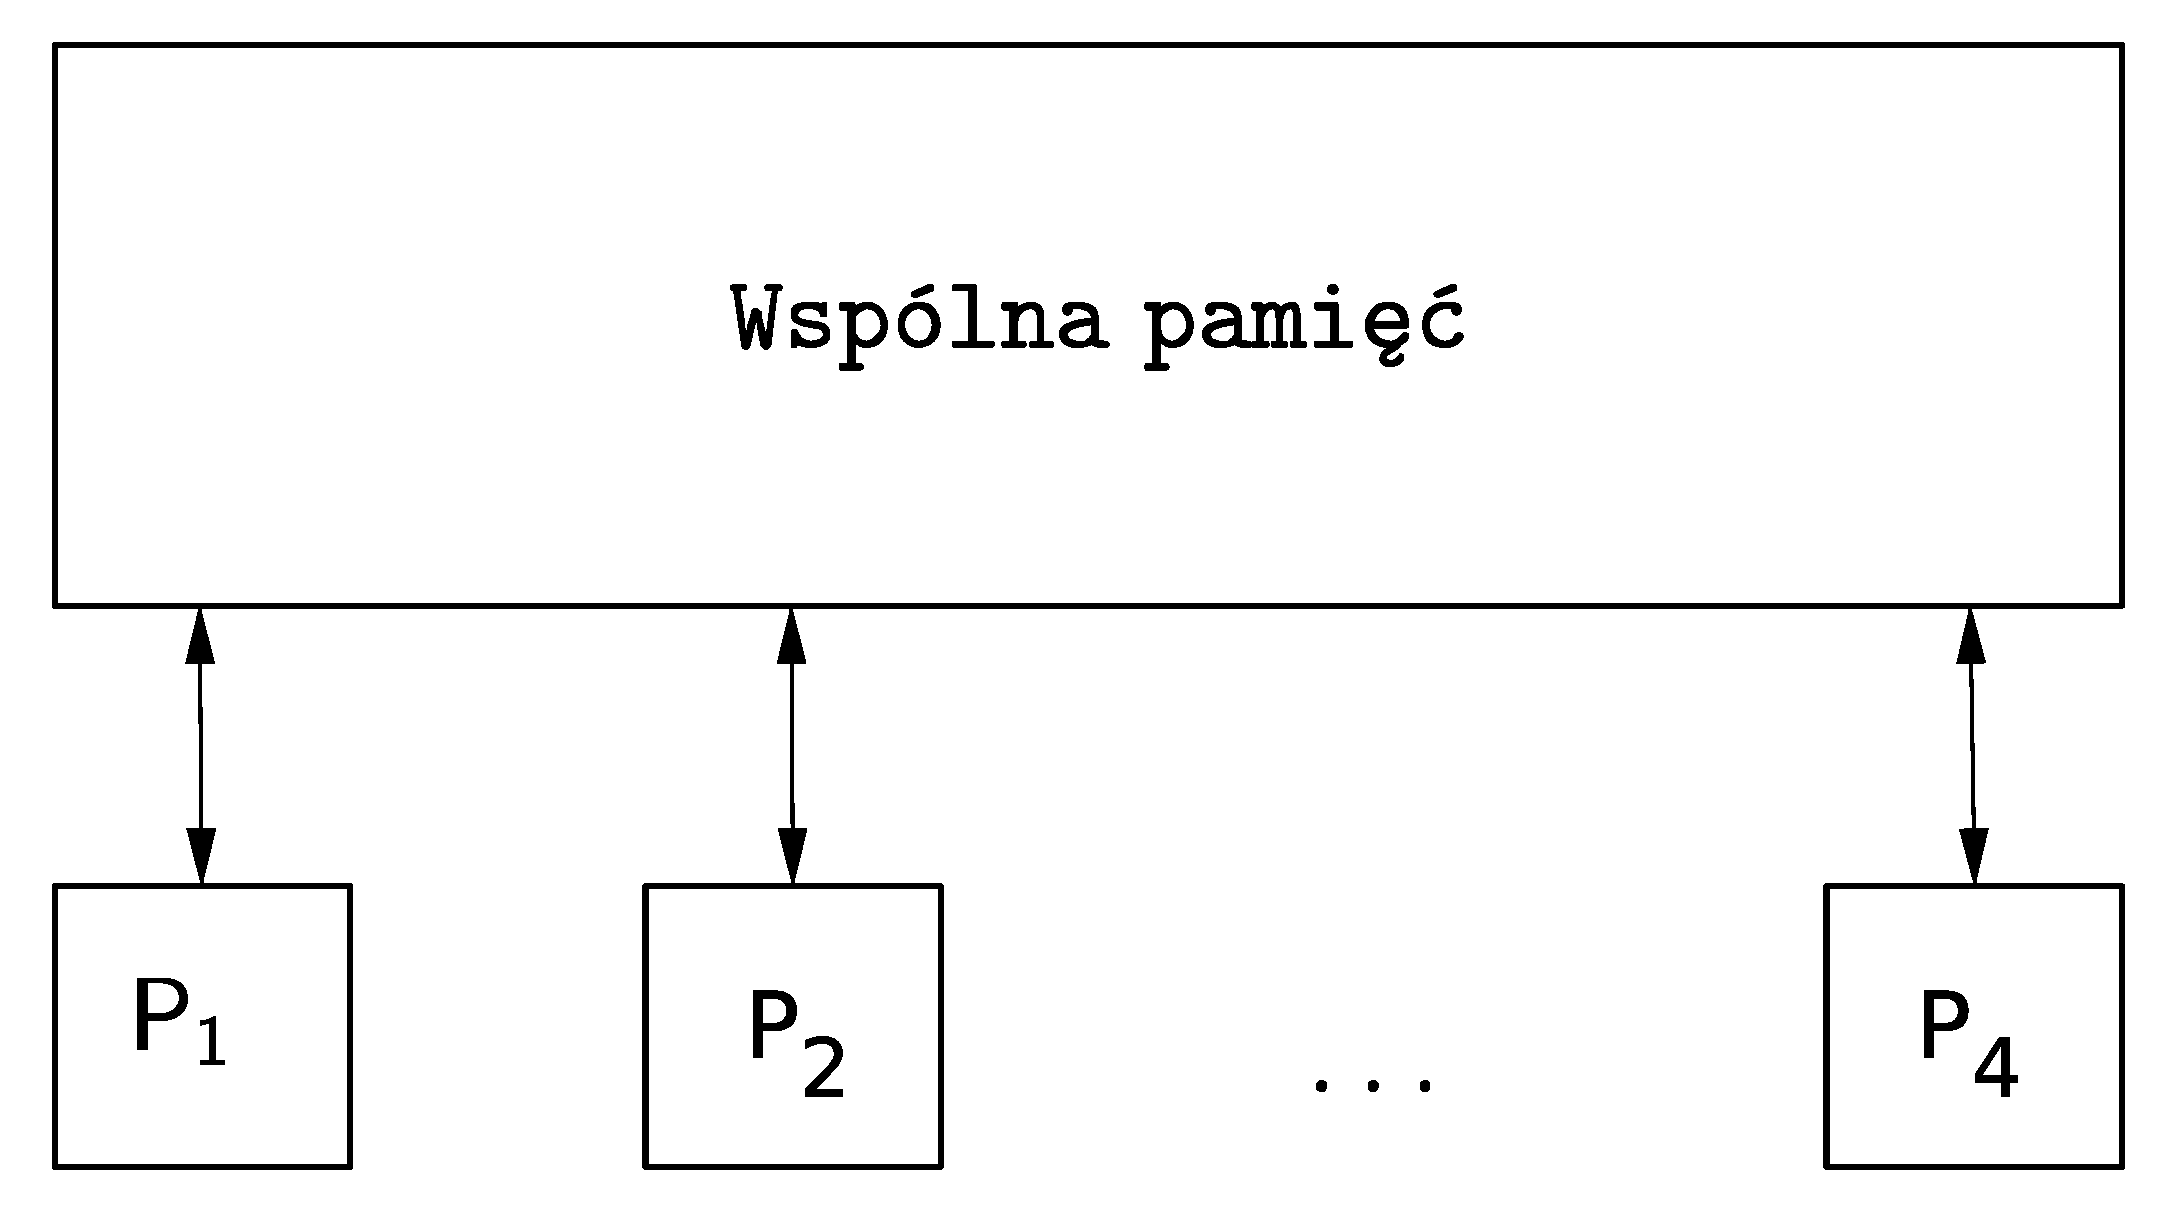
\includegraphics[width=20em]{./images/Rys4.eps}
\caption{Model wspólnej pamięci}
\label{fig:model_shared}
\end{figure}

\subsection{Model sieciowy}

Sieć możemy przedstawić modelowo jako graf \(G=(N,E)\), gdzie każdy węzeł \(i\in N\) oznacza procesor, a każda krawędź \((i, j) \in E\) – dwukierunkową komunikację między procesorami \(i\) i \(j\). Przyjmujemy, że każdy procesor ma swoją lokalną pamięć i nie ma żadnej pamięci współdzielonej przez procesory. Tak jak w przypadku modelu z pamięcią wspólną, operacje w sieci mogą być synchroniczne lub asynchroniczne.\\

W opisie algorytmów dla modelu sieciowego potrzebujemy zdefiniować dwie instrukcje do opisania komunikacji między procesorami.
\begin{enumerate}
 \item send\((X,i)\)
 \item receive\((X,j)\)
\end{enumerate}

Procesor \(P\) wykonujący instrukcję \textbf{send} wysyła kopię \(X\) do procesora \(P_i\), następnie natychmiast przechodzi do wykonywania kolejnej instrukcji.\\
Procesor \(P\) wykonujący instrukcję \textbf{receive} zatrzymuje wykonanie programu aż do chwili, gdy otrzyma dane z procesora \(P_j\), a następnie przechowuje dane w \(Y\) i kontynuuje wykonanie programu.\\



Procesory pracujące w sieci asynchronicznej zarządzają swoimi zadaniami przez wymianę komunikatów. Schemat taki nazywamy modelem wymiany komunikatów. Procesory te niekoniecznie muszą być ze sobą sąsiadujące. 

%\begin{definicja}[Routing]
%Proces dostarczania każdego komunikatu od źródła do przeznaczenia nazywmy routingiem.
%\end{definicja}

Charakterysuje ją kilka parametrów:

\begin{enumerate}
 \item średnica – maksymalna odległość (krawędziowa) między dowolną parą węzłów; im miejsza, tym lepiej.
 \item maksymalny stopień wierzchołka – maksymalna liczba łączy do dane procesora
 \item szerokość połowienia sieci – minimalna liczba krawędzi, które muszą zostać usunięty, aby podzielić ją na dwie równe podsieci
 \item spójność krawędziowa – minimalna liczba krawędzi, które muszą ulec awarii, aby sieć stała się niespójna
 \item koszt sieci – koszt wykonania, zarządzania i utrzymania połączeń między procesorami; w najprostrzym przypadku mierzony liczbą krawędzi
\end{enumerate}


\subsubsection{Sieć liniowa}
\begin{definicja}[Sieć liniowa]
Model składa się z \(p\) procesorów \(P_1, P_2, \dots, P_p\) połączonych ze sobą w ciąg, tzn. procesor \(P_i\) połączony jest z procesorem \(P_{i-1}\) i \(P_{i+1}\), o ile takie istnieją. Średnica takiej sieci wynosi \(p-1\), jej maksymalny stopień wynosi \(2\).\\
\end{definicja}
\begin{definicja}[Torus]
Sieć liniowa z połączonymi końcami.
\end{definicja}


\subsubsection{Sieć dwuwymiarowa}

Dwuwymiarowa sieć jest dwuwymiarową wersją sieci liniowej. Składa się ona z \(p=m^2\) procesorów ułożonych w siatkę \(m\times m\) taką, że procesor \(P_{i,j}\) jest połączony z procesorem \(P_{i\pm 1, j}\) i \(P_{i, j\pm 1}\).\\
Średnica takiej sieci złożonej z \(p=m^2\) procesorów wynos \(\sqrt{p}\) a jej maksymalny stopień \(4\)


\subsubsection{Sieć hipersześcienna}

\begin{definicja}{Kostka Boola}\\
Niech \(i_{d-1}i_{d-2}\dots i_{0}\), gdzie \(0\leq i \leq p-1\) będzie binarną reprezentacją \(i\). Wówczas procesor \({i}\) jest połaczony z procesorem \(P_{i^(j)}\), gdzie \(i^{(j)}=i_{d-1}\dots \overline{i_j} \dots i_0\) i \(\overline{i_j} = 1 - i_j\). Innymi słowy, dwa procesory są ze sobą połączone wtedy i tylko wtedy, gdy ich wskaźniki różnią się tylko jednym bitem.\\
\end{definicja}

Sieć w topologii hipersześcianu skłąda się z \(p=2^d\) procesorów połączonych w d-wymiarową kostkę Boola.\\

Hipersześcian ma strukurę rekursywną. Kostkę \(d\)-wymiarową możemy rozszerzyć do \(d+1\) wymiarów przez połączenie poszczególnych procesorów do \(d\)-wymiarowych kostek.\\

Średnica d-wymiarowego hipersześcianu wynosi \(d=\log{p}\). Jest tak ponieważ odległośc w grafie między dwoma procesorami \(P_i\) i \(P_j\) jest równa liczbie pozycji bitów, którymi wskaźniki \(i\) i \(j\) różnią się między sobą. Stąd jest ona mniejsza lub równa \(d\), a ponadto odległość między \(P_0\) a \(P_{2^d-1}\) wynosi d. Każdy węzeł jest stopnia \(d=\log{p}\).

\begin{figure}[h]
\centering
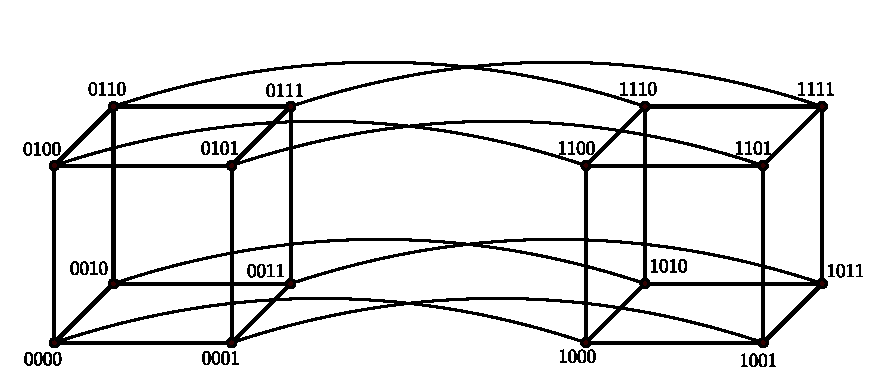
\includegraphics[width=36em]{./images/systolic.eps}
\caption{Sieć w topologii hipersześcianu}
\label{fig:systolic}
\end{figure}
\chapter{Klasyczne algorytmy mnożenia macierzy}
W swojej pracy \emph{,,Gaussian Elimination is not Optimal''} z 1969 roku \textsc{Volker Strassen} pokazał rekursyjny algorytm mnożenia macierzy kwadratowych wymiaru \(m2^k\) o złożoności \(\mathcal{O}(n^{2,81})\)\cite{Strassen68}. W przypadku macierzy \(2\times 2\) oznaczało to, że mnożenie można wykonać już za pomocą 7 mnożeń i 18 dodawań. Algorytm za sprawą \textsc{Shmuela Winograda} został zoptymalizowany\cite{Winograd}\cite{Loeckx1974} do najczęściej implementowanej dzisiaj postaci algorytmu \textsc{Strassena-Winograda} (implementacja zawiera się na przykład w bibliotece GEMMW\cite{Douglas94gemmw}). W przypadku macierzy \(2\times 2\) wykonuje on 7 operacji mnożenia i 15 dodawań\cite{DBLP:journals/corr/abs-1202-3173}.
\section{Algorytm naiwny}
Niech \(\mathbf{A}\), \(\mathbf{B}\in\mathbb{R}^{n\times n}\). Rozważmy algorytm sekwencyjny wyznaczania macierzy \(\mathbf{C}=\mathbf{AB}\) o złożoności \(\mathcal{O}(n^3)\).

\begin{algorithm}
\For{\(i\in\{1,2,\dots,n\}\)}{
\For{\(j\in\{1,2,\dots,n\}\)}{
\(\mathbf{C}(i,j)=0\)\;
\For{\(k\in\{1,2,\dots,n\}\)}{
\(\mathbf{C}(i,j)=\mathbf{C}(i,j)+\mathbf{A}(i,k) \mathbf{B}(k,j)\)\;
}}}
\caption{Sekwencyjny algorytm mnożenia macierzy}
\end{algorithm}
\newpage
\section{Algorytm ,,dziel i rządź''}
Dla danych macierzy wejściowych \(\mathbf{A}, \mathbf{B}\in\mathbb{R}^{n\times n}\) oraz macierzy wyjściowej \(\mathbf{C}\in\mathbb{R}^{n\times n}\) mamy:
\begin{align*}
\mathbf{A}& = \begin{bmatrix} A_{11}& A_{12} \\ A_{21}& A_{22} \end{bmatrix}&
\mathbf{B}& = \begin{bmatrix} B_{11}& B_{12} \\ B_{21}& B_{22} \end{bmatrix}&
\mathbf{C}& = \begin{bmatrix} C_{11}& C_{12} \\ C_{21}& C_{22} \end{bmatrix}
\end{align*}
gdzie
\begin{align}\label{eq:divide&conquer}
\begin{bmatrix} C_{11}& C_{12} \\ C_{21}& C_{22}\end{bmatrix}=
\begin{bmatrix} A_{11}& A_{12} \\ A_{21}& A_{22}\end{bmatrix}
\begin{bmatrix} B_{11}& B_{12} \\ B_{21}& B_{22}\end{bmatrix}
\end{align}
\eqref{eq:divide&conquer} możemy wyrazić inaczej:

\begin{equation}
\begin{split}
C_{11} &= A_{11}B_{11} + A_{12}B_{21}\\
C_{11} &= A_{11}B_{12} + A_{12}B_{22}\\
C_{21} &= A_{21}B_{11} + A_{22}B_{21}\\
C_{22} &= A_{21}B_{12} + A_{22}B_{22}
\end{split}
\end{equation}

Z powyższych konstatacji nasuwa się łatwy algorytm rekurencyjny.

\begin{algorithm}
\SetKwFunction{Multiply}{multiply}
\SetKwInOut{Input}{Dane wejściowe}
\SetKwInOut{Output}{Dane wyjściowe}
\SetKwProg{ParFor}{parfor}{}{}
\SetKwInOut{Help}{Dane pomocnicze}
\Multiply{\(\mathbf{A}, \mathbf{B}\)}\;
\Input{Macierze wejściowe \(\mathbf{A}, \mathbf{B}\) wymiaru \(n\)}
\Output{Macierz \(\mathbf{C}\)}
\Begin{
\uIf{n=1}{
\(C_{11}=A_{11}B_{11}\)
}
\Else{
\(C_{11}=\)
\Multiply{\(A_{11}B_{11}\)}+\Multiply{\(A_{12}B_{21}\)}\;
\(C_{12}=\) \Multiply{\(A_{11}B_{12}\)}+\Multiply{\(A_{12}B_{22}\)}\;
\(C_{21}=\) \Multiply{\(A_{21}B_{11}\)}+\Multiply{\(A_{22}B_{21}\)}\;
\(C_{22}=\) \Multiply{\(A_{21}B_{12}\)}+\Multiply{\(A_{22}B_{22}\)}\;
}
\Return{C}
}
\end{algorithm}
\section{Algorytm Cannona}
\cite{Cannon:1969:CCI:905686}
\section{Algorytm Strassena}
Niech \(A\) i \(B\) będą macierzami \(m2^k\times m2^k\). Definiując następujące macierze pomocnicze
\begin{align*}
H_1 &= (A_{11}+A_{22})(B_{11}+B_{22})&
 H_2 &= (A_{21}+A_{22})B_{11}\\
H_3 &= A_{11}(B_{12} + A_{22})&
 H_4 &= A_{22}(B_{21} + A_{11})\\
H_5 &= (A_{11}+A_{12})B_{22}&
 H_6 &= (A_{21} + A_{11})(B_{11} + B_{12}) \\
H_7 &= (A_{12}-A_{22})(B_{21}+B_{22}) 
\end{align*}
otrzymujemy
\begin{align}
C = \begin{bmatrix}
H_1+H_4-H_5+H_7& H_3+H_5\\
H_2+H_4& H_1+H_3-H_2+H_6
\end{bmatrix}
\end{align}

\section{Algorytm Strassena-Winograda}
Dla danych macierzy wejściowych \(\mathbf{A}, \mathbf{B}\) oraz macierzy wyjściowej \(\mathbf{C}\) mamy
\begin{align*}
\mathbf{A}& = \begin{bmatrix} A_{11}& A_{12} \\ A_{21}& A_{22} \end{bmatrix}&
\mathbf{B}& = \begin{bmatrix} B_{11}& B_{12} \\ B_{21}& B_{22} \end{bmatrix}&
\mathbf{C}& = \begin{bmatrix} C_{11}& C_{12} \\ C_{21}& C_{22} \end{bmatrix}
\end{align*}

Następnie ustalmy odpowiednio po siedem kombinacji liniowych \(T_i\), \(S_i\), \(i\in \{1, 2, \dots,7\}\) dla każdej z podmacierzy \(\mathbf{A}\) i \(\mathbf{B}\).

\begin{align*}
T_0& = A_{11}& S_0 &= B_{11}\\
T_1& = A_{12}& S_1 &= B_{21}\\
T_2& = A_{21} + A_{22}& S_2 &= B_{12}+B_{11}\\
T_3& = T_2 - A_{12}& S_3 &= B_{22}-S_2\\
T_4& = A_{11}-A_{21}& S_4 &= B_{22}-B_{12}\\
T_5& = A_{12}+T_3& S_5 &= B_{22}\\
T_6& = A_{22}& S_6 &= S_3-B_{21}
\end{align*}
oraz
\begin{align*}
Q_0& = T_{0}S_{0}& U_1 &= Q_{0} + Q_{3}\\
Q_1& = T_{1}S_{1}& U_2 &= U_{1} + Q_{4}\\
Q_2& = T_{2}S_{2}& U_3 &= U_{1} + Q_{2}\\
Q_3& = T_{3}S_{3}& C_{11} &= Q_{0} + Q_{1}\\
Q_4& = T_{4}S_{4}& C_{12} &= U_{3} + Q_{5}\\
Q_5& = T_{5}S_{5}& C_{21} &= U_{2} - Q_{6}\\
Q_6& = T_{6}S_{6}& C_{22} &= U_{2} + Q_{2}
\end{align*}

Jest to jeden krok metody Strassena-Winograda. Algorytm jest rekursywny ponieważ może być użyty ponownie dla wyznaczenia \(Q_i,\,i\in\{0,1,\dots,6\}\)

W praktyce stosuje się tylko kilka kroków algorytmu Strassena-Winegrada\cite{DBLP:journals/corr/abs-1202-3173}. Złożoność obliczeniową \(O(n^{w_0})\) algortytmu oznacza, że jego wykonanie zatrzymuje się po osiągnięciu macierzy wymiaru \(1\times 1\).

\chapter{Równoległe algorytmy mnożenia macierzy}
\section{Algorytm w modelu PRAM}
\subsubsection{Algorytm sumowania}
Niech dany będzie tablica \(A\) \(n=2^k\) liczb i maszyna PRAM z n-procesorami \(\{P_1, P_2, \dots, P_n\}\). Każdy z procesorów wykonuje synchronicznie poniższy algorytm

\label{alg:crew_pram_sum}
\begin{algorithm}[H]
\SetKwFunction{Gread}{global read}
\SetKwFunction{Gwrite}{global write}
\SetKwInOut{Input}{Dane wejściowe}\SetKwInOut{Output}{Dane wyjściowe}
\Input{Tablica \(A\) długości \(n=2^k\) przechowywana w pamięci wspólnej. Każdy procesor ma zainicjalizowane zmienne lokalne \(n\) oraz identyfikator \(i\)}
\Output{Suma \(S\) wartości tablicy \(A\). Tablica \(A\) nie ulega zmianie}
\begin{enumerate}
 \item \Gread{A(i), a}
 \item \Gwrite(a, B(i))
 \item for \(h = 1\) to \( \log{n}\) do\\
	 if \(i \leq n/2^k\) then\\
	 \Gread{B(2i-1), x}\\
	 \Gread{B(2i),y}\\
	 Set z:= x + y\\
	 \Gwrite(z, B(i))\\
 \item \(if(i=1)\) then \Gwrite{z, S}
\end{enumerate}
\caption{Algorytm sumowania w PRAM\label{alg:pram_sum}}
\end{algorithm}

Przypadek dla \(n=8\) ilustruje rysunek \ref{fig:pram_sum}. W pierwszym i drugim kroku kopia B tablicy A jest tworzona w pamięci wspólnej. 
Zadania obliczeniowe w kroku 3 są na podstawie wyważonego drzewa binarnego, którego liście odpowiadają elementom tablicy A. Procesor odpowiedzialny za wykonanie za wykonanie operacji jest określony przez indeks poniżej węzła reprezentującego tę operację. Zauważmy, że procesor \(P_1\), odpowiedzialny za ustawianie wartości \(B(1)\) i zapisywanie sumy \(S\), jest zawsze aktywny w trakcie wykonywania algorytmu, podczas gdy procesory \(P_5, P_6, P_7, P_8\) są aktywne tylko podczas kroków 1 i 2.

\begin{uwaga}
Pomijamy szczegóły operacji dotyczących dostępu do pamięci. Operacje postaci \texttt{Ustaw A:=B+C}, gdzie A, B i C są zmiennymi wspólnymi będziemy interpretować jako ciąg instrukcji\\
\begin{algorithm}[H]
\SetKwFunction{Gread}{global read}
\SetKwFunction{Gwrite}{global write}
\Gread{B, x}\;
\Gread{C, y}\;
\texttt{Ustaw} z:= x + y\;
\Gwrite{z,A}\;
\end{algorithm}
\end{uwaga}

\begin{figure}[h]
\centering
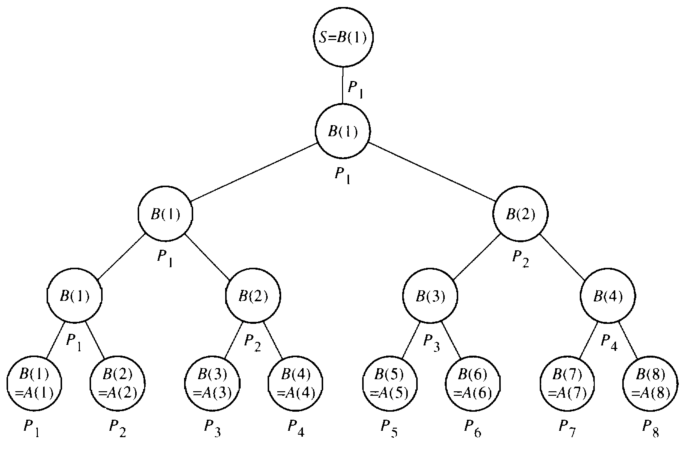
\includegraphics[width=34em]{./images/pram_sum}
\caption{Algorytm sumowania ośmiu elementów w modelu PRAM z osmioma procesorami. Każdy wewnętrzny wierzchołek grafu reprezentuje operację sumowania.}
\label{fig:pram_sum}
\end{figure}


\subsubsection{Algorytm mnożenia}
Rozważmy problem obliczenia iloczynu \(\mathbf{C}\) dwóch macierzy \(\mathbf{A}\), \(\mathbf{B}\in\mathbb{R}^{n\times n}\), gdzie \(n=2^k\), dla pewnego \(k\in\mathbf{N}\). Załóżmy, że dysponujemy \(n^3\) procesorami \(P_{i,j,l}\), \(1\leq i, j, l \leq n\) maszyny PRAM. Wówczas dla każdej pary \((i, j)\), n procesorów \(P_{i,j,l}\), gdzie \(1\leq l \leq n\), oblicza sumę \(\sum_{l=1}^{n}A(i,l)B(l,j)\) w myśl algorytmu \ref{alg:pram_sum}.\\

\label{alg:crew_pram_multiplication}
\begin{algorithm}[H]
\SetKwData{Left}{left}\SetKwData{This}{this}\SetKwData{Up}{up}
\SetKwFunction{Union}{Union}\SetKwFunction{FindCompress}{FindCompress}
\SetKwInOut{Input}{wejście}\SetKwInOut{Output}{wyjście}
\Input{Macierze \(\mathbf{A}\), \(\mathbf{B}\in\mathbb{R}^{n\times n}\), gdzie \(n=2^k\), dla pewnego \(k\in\mathbf{N}\) przechowywanych we wspólnej pamięci. Lokalnie zainicjalizowane zmienne to \(n\) i trójka wskaźników \((i, j, l)\)}
\Output{Iloczyn \(\mathbf{C=AB}\) w pamięci współdzielonej}
\begin{enumerate}
 \item \( \mathtt{Oblicz}\quad C'(i,j,l) = A(i,l)B(l,j) \)
 \item for \(h = 1\) to \( \log{n}\) do\\
 if \(l \leq n/2^k\) then \texttt{Ustaw} \(C'(i,j,l):=C'(i,j,2l-1)+C'(i,j,2l)\)
 \item \(if(l=1)\) then \texttt{Ustaw} \(C(i,j):=C'(i,j,1)\)
\end{enumerate}
\caption{Algorytm mnożenia macierzy w modelu PRAM\label{alg:pram_pseudokod}}
\end{algorithm}

\begin{uwaga}
Algorytm \ref{alg:crew_pram_multiplication} wymaga równoległego odczytu ponieważ w trakcie wykonania kroku (1) procesory \(P_{i,l,k}\) mogą równocześnie odczytywać te same dane. Przykładowo procesory \(P_{i,1,l},P_{i,2,l},\dots,P_{i,n,l}\) w trakcie wykonywania kroku (1) wszystkie wymagają dostępu do \(A(i,l)\).
\end{uwaga}

\section{Algorytmy w modelu sieciowym}
%\subsection{Jednowymiarowy torus}
%\label{alg:entorus_asynch_mesh}
%\begin{algorithm}[H]
%\SetKwInOut{Input}{Dane wejściowe}
%\SetKwInOut{Output}{Dane wyjściowe}
%\SetKwProg{ParFor}{parfor}{}{}
%\SetKwInOut{Help}{Dane pomocnicze}
%\Input{
%\begin{enumerate}
%\item podmacierze \(b=a\left((i-1)r+1\dots ir,1\dots n\right)\)
%\item \(r=\frac{n}{p}\)
%\item wektor \(x[1\dots n]\) umieszczone w procesorach \(P_i\) pracujących asynchronicznie, \(1\leq i  \leq p\) połączonych w pierścień
%\item zmienne lokalne w każdym procesorze \(P_i\) służace do przechowywania rozmiaru \(n\) oraz numeru procesora w postaci zmiennej \(i\)
%\end{enumerate}
%
%\Output{Iloczyn \(z=ax\) umieszczony w procesorze \(P_i\)}
%\Begin
%{
%\tcp*[f]{Oblczanie wektora \(y=bx\) przez procesory \(P_i, 1\leq i \leq p\)}\;
%
%\For{\(i=1 \quad \KwTo \quad n/p\)}
%{
%y[k]:=b[k,1]*x[1]\;
%\For{\(j:=1 \quad \KwTo \quad n\)}
%{
%y[k]:=y[k]+b[k,j]*x[j]\;
%}
%}
%\uIf{i:=1}{
%\(\mathtt{send}(y,prawy)\)\;
%}
%\Else{
%\(\mathtt{receive}(z[1..(i-1)r],lewy)\)\;
%\(z[1..ir]:=z[1..(i-1)]r\,||\,y\)\tcp*[f]{dopisanie wektora y}\;
%\(\mathtt{send}(z[1..ir],\,prawy)\)\;
%}
%\If{\(i=1\)}{
%\(\mathtt{receive}(z[1..n],\, lewy)\)\;
%\tcp*[f]{odebranie przez procesor \(P_1\) końcowego wyniku}\;
%}
%}
%}
%\caption{Algorytm mnożenia macierzy przez wektor w jednowymiarowym torusie}
%\end{algorithm}


\subsection{Algorytm w dwuwymiarowym torusie}
\begin{algorithm}[H]
\SetKwFunction{Prawy}{prawy}
\SetKwFunction{Dol}{dół}
\SetKwInOut{Input}{Dane wejściowe}
\SetKwInOut{Output}{Dane wyjściowe}
\SetKwProg{ParFor}{parfor}{ do}{end}
\SetKwInOut{Help}{Dane pomocnicze}
%\begin{multicols*}{2}
\Input{\begin{enumerate}
\item macierze \(a\left[1..n,\,1..n\right]\) i \(b\left[1..n,\,1..n\right]\), których elementy \(a\left[i,\,j\right]\) umieszczone są w pamięciach lokalnych procesorów \(P_{i,j}\)
\item zmienna lokalna w każdym procesorze służące do przechowyuwania rozmiaru \(n\)
\item zmienne lokalne \(i\) oraz \(j\) przechowujące numer procesora
\end{enumerate}
}

\Help{
zmienna lokalna \(k\) w każdym procesorze \(P_{i,j}\)
}
\Output{
\begin{enumerate}
\item iloczyn macierzy \(c=ab\)
\item elementy macierzy \(c[i,j]\) umieszczone w lokalnych zmiennych \(c\) procesorów \(P_{i,j}\)
\end{enumerate}
}
%\end{multicols*}
\Begin{
\For{\(k:=2\) \To \(n\)}{
\ParFor{\(P_{i,j},\, 1\leq i,\,j\leq n\) }{
\If{\(k \leq i\) }{
\(a\Longleftarrow\)\Prawy{\(a\)} \tcp*[r]{Przemieszczenie wierszy  \(a\)}
\tcp*[r]{macierzy cyklicznie w lewo}
}
\If{\(k\leq j\)}{
\(b\):=\Dol{\(b\)}\tcp*[f]{Przemieszczenie kolumn macierzy \(b\)}
\tcp*[r]{cyklicznie w górę}
}
}
}
\tcp*[h]{Obliczanie iloczynu macierzy \(a\) i \(b\)}\;
\For{\(k:=1\)\To \(n\)}{
\ParFor{\(P_{i,j}, 1\leq i,\, j\leq n\)} {
\uIf{\(k=1\)} {
c:=a*b\;
}
\Else {
a\(\Longleftarrow\)\Prawy{a}; b\(\Longleftarrow\)\Dol{b}; c:=c+a*b\;
}
}
}
}
\end{algorithm}

\subsection{Algorytm systoliczny w sieci dwuwymiarowej}

Rysunek \ref{fig:systolic_mesh} przedstawia możliwy schemat obliczenia iloczynu \(AB = C\) w myśl paradygmatu systolicznego. Wiersze macierzy \(A\) są wprowadzane synchroniczne skośnie od lewej strony sieci; kolumny macierzy \(B\) są wprowadzane synchronicznie skośnie od góry sieci.\\
Gdy procesor \(P_{i,j}\) odbierze dwie dane wejściowe \(A(i, l)\) i \(B(l,j)\), to przeprowadza operację \(C(i,j):=C(i,j+A(i,l)(B(l,j)\); po tym przesyła \(A(i,l)\) do swojego prawego sąsiada, a \(B(l,j)\) do sąsiada poniżej.

Po \(O(n)\) krokach, każdy procesor \(P_{i,j}\) będzie miał szukaną wartość \(C(i,j)\).\\

Algorytmy systoliczne pracują całkowicie synchronicznie; w każdej jednostce czasu, procesor otrzymuje dane od pewnego sąsiada, przeprowadza na nich lokalne obliczenia i następnie wysyła dane do któregoś swojego sąsiada.

\begin{figure}[h]
\centering
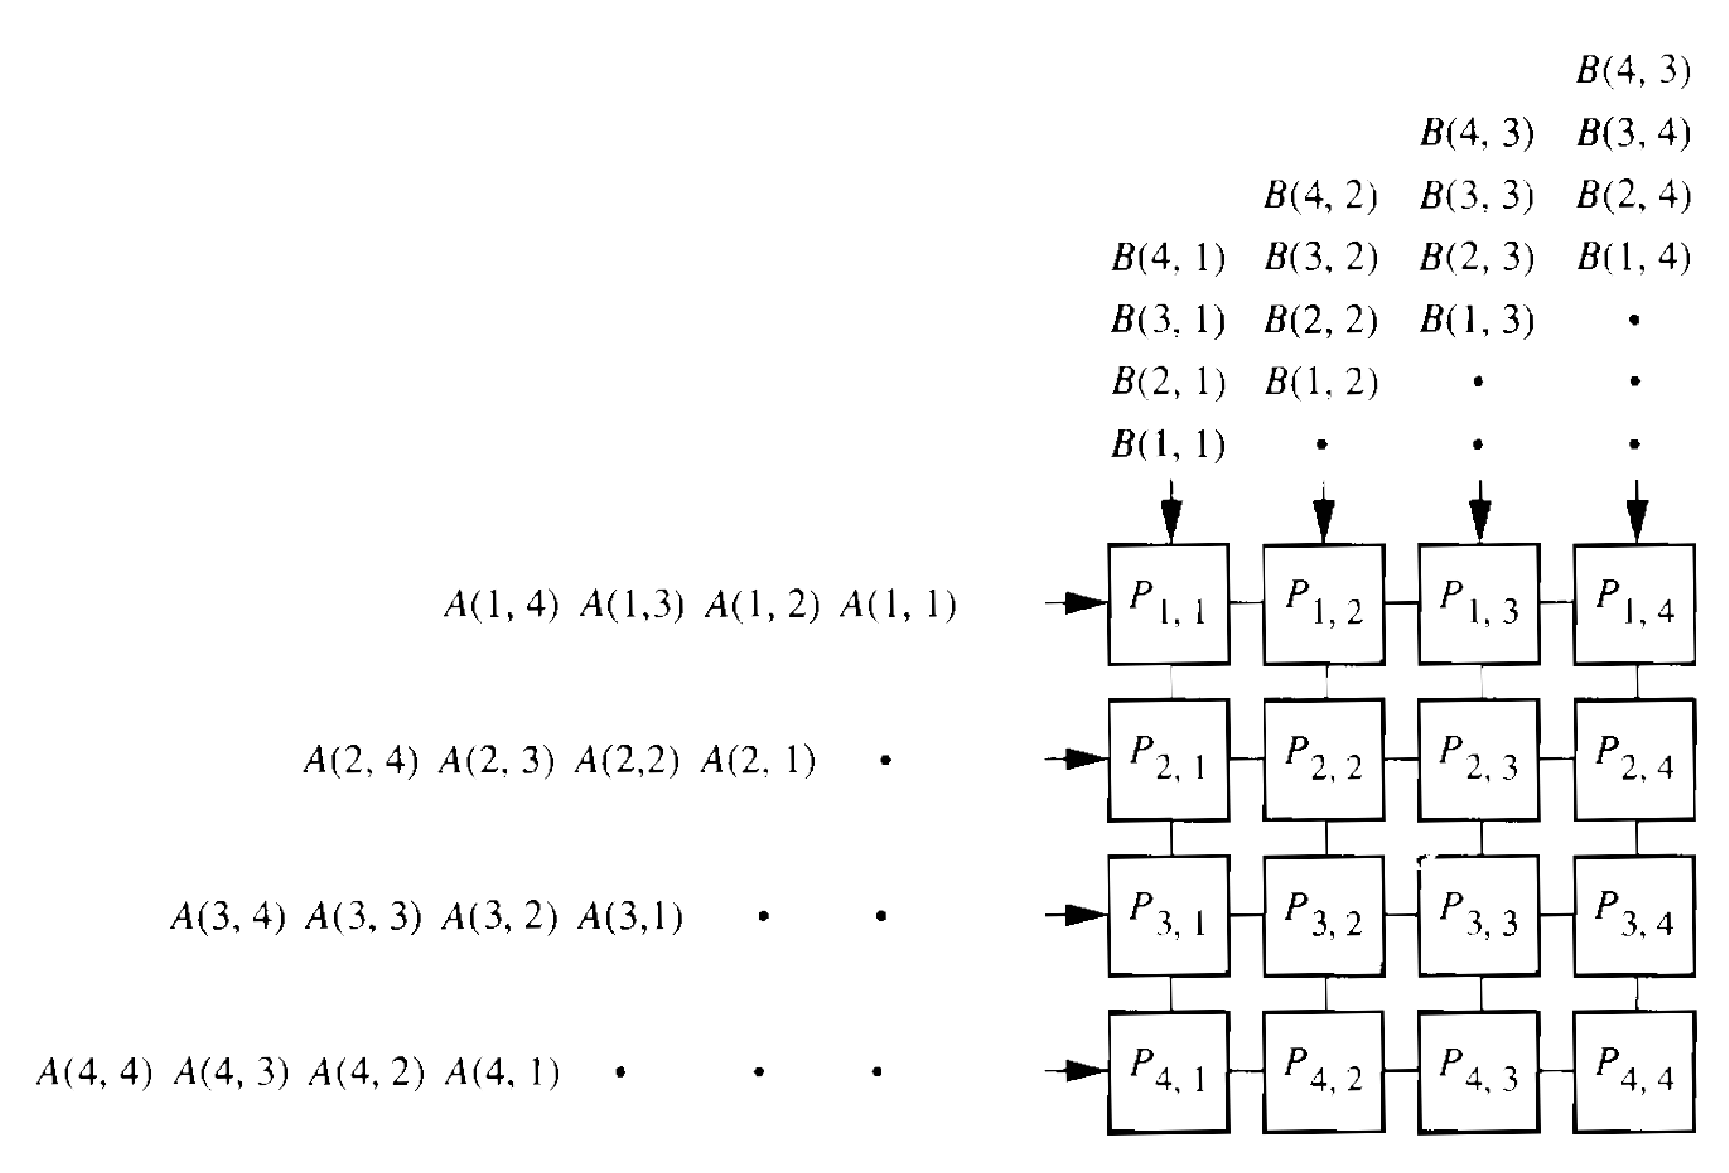
\includegraphics[width=30em]{./images/systolic2.eps}
\caption{Mnożenie macierzy w modelu sieciowym za pomocą algorytmu systolicznego. Wiersze macierzy \(\mathbf{A}\) są synchronicznie umieszczane w sieci od lewej strony, podczas, gdy równocześnie ,,od góry'' umieszczane są synchronicznie kolumny macierzy \(\mathbf{B}\). Gdy elementy \(A(i,l)\) i \(B(l,j)\) są dostępne na procesorze \(P_{i,j}\), wykonywane jest działanie \(C(i,j)=C(i,j)+A(i,l)B(l,j)\), \(A(i,l)\) zostaje wysłany do procesora \(P_{i,j+1}\) (o ile taki istnieje) oraz \(B(l,j)\) zostaje wysłany do procesora \(P_{i+1,j}\) (o ile taki istnieje).}
\label{fig:systolic_mesh}
\end{figure}

\subsection{Algorytm w topologii hipersześcianu}
\subsubsection{Rozgłaszanie ,,jednego do wszystkich'' w hipersześcianie}
Rozważmy problem rozgłaszania elementu \(X\) przechowywanego w rejestrze \(D(0)\) procesora \(P_0\) do wszystkich procesorów \(P_i\) p-procesorowego hipersześcianu, gdzie \(p=2^d\).

Algorytm polega na przechodzeniu z podkostek najniższego wymiaru, kolejno do najwyższego w \(d\) iteracjach. Pierwsza iteracja polega na wysłaniu kopii \(X\) przez procesor \(P_0\) do procesora \(P_1\). W drugiej iteracji procesor \(P_0\) i \(P_1\) wysyłają kopię \(X\) do \(P_2\) i \(P_3\) odpowiednio. Analogiczną operację przeprowadza się d-razy.




\begin{algorithm}\label{alg:broadcast_one_many}
\SetKwFunction{Prawy}{prawy}
\SetKwFunction{Dol}{dół}
\SetKwInOut{Input}{Dane wejściowe}
\SetKwInOut{Output}{Dane wyjściowe}
\SetKwProg{ParFor}{parfor}{ do}{end}
\SetKwInOut{Help}{Dane pomocnicze}
\Input{Procesor \(P_0\) z \(p=2^d\)-procesorowego synchronicznego hipersześcianu przechowuje element danych \(X\) w rejestrze \(D(0)\).}
\Output{\(X\) jest rogłaszany do wszystkich procesorów tak, że \(D(i)=X\), gdzie \(1\leq i \leq p-1\)}
\tcp*[l]{Algorytm dla procesora \(P_i\)}
\Begin{
\For{\(l=0\) \To \(d-1\)}{
\If{\(0\leq i \leq 2^l-1\)}{
Ustaw \(D(i^l):=D(i)\)\;
}
}
}
\caption{Algorytm rozgłaszania w sieci hipersześciennej}
\end{algorithm}


Algorytm \ref{alg:broadcast_one_many} ma złożoność równoległą \(\mathcal{O}(\log{p})\)

\subsubsection{Algorytm mnożenia}
Rozważmy problem mnożenia macierzy \(AB = C\) w synchronicznym hipersześcianie z \(p=n^3\) procesorów, gdzie wszystkie macierze są wymiaru \(n\times n\).\\
Niech \(n=2^q\) i stąd \(p=2^{3q}\). Przypiszmy procesorom indeksy \((l,i,j)\) takie, że \(P_{l,i,j}\) oznacza procesor \(P_r\), gdzie \(r=ln^{2}+in+j\). Innymi słowy, rozkładając indeks \(r\) binarnie otrzymuje, że \(q\) najbardziej znaczących bitów odpowiada indeksowi \(l\), następne \(q\) najbardziej znaczących bitów odpowiada indeksowi \(i\) i ostatecznie \(q\) najmniej znaczących bitow odpowiada wskaźnikowi \(j\). W szczególności, jeśli ustalimy dowolną parę wskaźników spośród \(l\), \(i\) oraz \(j\) oraz będziemy przechodzili z pozostałym wskaźnikiem po wszystkich jego możliwych wartościach, otrzymamy podkostkę wymiaru \(q\).\\

Wejściowy ciąg \(A\) jest zapamiętany w podkostce wyznaczonej przez procesory \(P_{l,i,0}\), gdzie \(0\leq l, i \leq n-1\), tak, że \(A(i,l)\) jest zapamiętane w procesorze \(P_{l,i,0}\).\\
Podobnie ciąg B jest zapamiętany w podkostce procesorów \(P_{l,0,j}\), gdzie procesor \(P_{l,0,j}\) zapamiętuje \(B(l,j)\).\\
Celem jest obliczeniem \(C(i,j)=\sum_{l=0}^{n-1}A(i,l)B(l,j)\) dla \(0\leq i, j\leq n-1\). Algorytm składa się z trzech etapów:
\begin{enumerate}
 \item Dane wejściowe są rozdystrybuowane tak, że procesor \(P_{l,i,j}\) pamięta \(A(i,l)\) i \(B(l,j)\) dla \(0\leq l, i, j \leq n-1\).
 \item Procesor \(P_{l,i,j}\) oblicza iloczyn \(C'(l,i,j)=A(i,l)B(l,j)\) dla wszystkich \(0\leq i, j, l \leq n-1\).
 \item Dla wszystkich \(0\leq i, j \leq n-1\) procesorów \(P_{l,i,j}\), gdzie \(0\leq l\leq n-1\), obliczają sumę \(C(i,j)=\sum_{i=0}^{n-1} C'(l,i,j)\)
\end{enumerate}

Implementacja pierwszego etapu składa się z dwóch części. W pierwszej z nich \emph{rozgłaszamy}, dla każdego \(i, l, A(i,l)\), z procesora \(P_{i,l,0}\) do \(P_{l,i,})\) dla \(0\leq j \leq n-1\). Ponieważ zbiór procesorów \(\{P_{l,i,j}|0\leq j \leq n-1\}\) wyznacza q-wymiarową kostkę dla każdej z par \(i\) oraz \(l\), możemy użyć \textbf{algorytmu rozgłaszania}, żeby rozgłosić \(A(i,l)\) od procesora \(P_{l,i,0}\) do wszystkich procesorów \(P_{l,i,j}\).
W drugiej części każdy element \(B(l,j)\) przechowywany w procesorze \(P_{l,0,j}\) jest rozgłaszany do procesorów \(P_{l,i,j}\) dla wszystkich \(0\leq i \leq n-1\). Pod koniec procesor \(P_{l,i,j}\) będzie przechowywał dwie wartości: \(A(i,l)\) i \(B(l,j)\). Używając algorytmu (tutaj referencja) etap pierwszy ma równoległą złożonośc czasową \(O(\log{n})\).

Drugi etap polega na wykonywaniu pojedyńczych mnożeń na każdym z procesorów \(P_{l,i,j}\). Stąd etap na etap ten składa się tylko jeden równoległy krok obliczeniowy. Pod koniec procesor \(P_{l,i,j}\) przechowuje \(C'(l,i,j)\).

Trzeci etap polega na obliczeniu \(n^2\) sum \(C(i,j)\). Wartości \(C'(l,i,j)\) każdej z sum znajudują się w q-wymiarowym hipersześcianie \(\{P_{l,i,j}\,|\,0\leq l\leq n-1\}\). Obliczanie takich sum ma równoległą złożoność czasową \(O(\log{n}\). Procesor \(P_{0,i,j}\) będzie przechowywał wartość \(C(i,j)\) iloczynu.

Wobec powyższych iloczyn macierzy wymiaru \(n \times n\) w sieci hipersześciennej może być obliczony w czasie \(O(\log{n})\) dysponując \(n^3\) procesorami.
\subsection{Algorytm Cannona w dwuwymiarowej sieci}
\cite{communication_efficient}
\subsection{Algorytm 2.5D}
\cite{Solomonik:EECS-2011-72}
\subsection{Algorytm 3D}
\cite{communication_efficient}
\subsection{Równoległy algorytm Strassena CAPS}
\cite{DBLP:journals/corr/abs-1202-3173}

\chapter{Interfejsy programowania równoległego}
\section{MPI}
\section{OpenMP}
\section{Cilk++}

\chapter{Implementacja wybranych algorytmów}
\section{MPI}
\section{OpenMP}
\section{Cilk++}

\bibliographystyle{unsrt}
\bibliography{bibdb}

\end{document}